% ==========================================================================
%  Prosjekt 1: Telegraflikningen
%  Kompiler med:  latexmk -pdf rapport.tex   (eller pdflatex to ganger)
%  Figurer og tabeller lages av  ../kode/lag_figurer.py
% ==========================================================================
\documentclass[11pt,a4paper]{article}

\usepackage[T1]{fontenc}
\usepackage[utf8]{inputenc}
\usepackage[norsk]{babel}
\usepackage{lmodern}
\usepackage{microtype}
\usepackage[a4paper,margin=2.5cm]{geometry}
\usepackage{amsmath,amssymb}
\usepackage{graphicx}
\usepackage{booktabs}
\usepackage{array}
\usepackage{caption}
\usepackage{float}
\usepackage[separate-uncertainty]{siunitx}
\usepackage{circuitikz}
\usepackage{fancyhdr}
\usepackage{listings}
\usepackage{xcolor}
\usepackage{etoolbox}
\usepackage[hidelinks]{hyperref}

% ---------- Opplysninger til forsiden (fyll inn) ---------------------------
\newcommand{\Emne}{[Emnekode og emnenavn]}
\newcommand{\Forfattere}{[Navn 1], [Navn 2], [Navn 3]}
\newcommand{\Gruppe}{[Gruppenummer]}
\newcommand{\Klasse}{[Klasse]}
\newcommand{\DatoUtfort}{[Periode, f.eks. 30.09.--13.10.2026]}
\newcommand{\DatoLevert}{14.10.2026}

% ---------- Tall og enheter -------------------------------------------------
\sisetup{
  output-decimal-marker = {,},
  exponent-product      = \cdot,
  number-unit-product   = {},
  per-mode              = symbol,
  group-minimum-digits  = 5,
  range-phrase          = {--},
  range-units           = single,
}
\newcommand{\DD}{5e+08}
\newcommand{\GC}{0.0004}
\newcommand{\LHeaviside}{123}
\newcommand{\Lpupin}{48.7}
\newcommand{\VLdc}{0.214}
\newcommand{\aB}{2e+06}
\newcommand{\aC}{4e+06}
\newcommand{\aD}{4e+07}
\newcommand{\dalfaPupin}{0.15}
\newcommand{\dalfaUten}{1.8}
\newcommand{\dtauPupin}{0.039}
\newcommand{\dtauUten}{0.16}
\newcommand{\feilC}{4.7e-05}
\newcommand{\fpuls}{48}
\newcommand{\frontD}{4.5e-05}
\newcommand{\ncD}{6.37}
\newcommand{\tfemtiD}{5.49}
\newcommand{\tfemtiDdiff}{5.5}
\newcommand{\toppB}{0.377}
\newcommand{\toppBteori}{0.368}
\newcommand{\toppC}{0.135}
\newcommand{\vgmaks}{1.089}
\newcommand{\wvgmaks}{0.577}

% Primitiv \input, slik at genererte tabellrader kan stå rett før \bottomrule
\makeatletter
\newcommand{\tabellrader}[1]{\@@input #1 }
\makeatother

% ---------- Nummerering -----------------------------------------------------
\numberwithin{equation}{section}
\numberwithin{figure}{section}
\numberwithin{table}{section}
\captionsetup{font=small, labelfont=bf, labelsep=period}
\addto\captionsnorsk{%
  \renewcommand{\figurename}{Figur}%
  \renewcommand{\tablename}{Tabell}%
  \renewcommand{\contentsname}{Innholdsfortegnelse}%
  \renewcommand{\refname}{Litteraturreferanser}%
}
% Referanselista blir et nummerert kapittel i innholdsfortegnelsen
\patchcmd{\thebibliography}{\section*{\refname}}{\section{\refname}}{}{}

% ---------- Topptekst og bunntekst -------------------------------------------
\pagestyle{fancy}
\fancyhf{}
\fancyhead[L]{\small Prosjekt 1: Telegraflikningen}
\fancyhead[R]{\small Gruppe \Gruppe}
\fancyfoot[C]{\thepage}
\renewcommand{\headrulewidth}{0.4pt}
\setlength{\headheight}{14pt}

% ---------- Programkode -----------------------------------------------------
\lstset{
  language=Python,
  basicstyle=\ttfamily\scriptsize,
  keywordstyle=\color{blue!60!black}\bfseries,
  commentstyle=\color{green!40!black},
  stringstyle=\color{red!50!black},
  numbers=left, numberstyle=\tiny\color{gray}, numbersep=6pt,
  frame=single, rulecolor=\color{gray!50},
  breaklines=true, showstringspaces=false, columns=fullflexible,
  literate={æ}{{\ae}}1 {ø}{{\o}}1 {å}{{\aa}}1 {Æ}{{\AE}}1 {Ø}{{\O}}1 {Å}{{\AA}}1,
}

% ---------- Snarveier ---------------------------------------------------------
\newcommand{\dd}{\mathrm{d}}
\newcommand{\jj}{\mathrm{j}}
\newcommand{\pd}[2]{\frac{\partial #1}{\partial #2}}
\newcommand{\pdd}[2]{\frac{\partial^2 #1}{\partial #2^2}}
\renewcommand{\Re}{\operatorname{Re}}
\renewcommand{\Im}{\operatorname{Im}}

\setlength{\parindent}{0pt}
\setlength{\parskip}{0.6em}

\begin{document}

% ==========================================================================
%  FORSIDE
% ==========================================================================
\begin{titlepage}
  \centering
  \vspace*{2.5cm}
  {\large PROSJEKTRAPPORT\par}
  \vspace{0.4cm}
  {\large Prosjekt 1 \quad -- \quad Tema 3: Telegraflikningen. Dispersjon.\par}
  \vspace{1.6cm}
  {\LARGE\bfseries Telegraflikningen\par}
  \vspace{0.4cm}
  {\Large Bølger, demping og dispersjon på elektriske overføringslinjer\par}
  \vspace{2.2cm}
  \begin{tabular}{>{\raggedleft\arraybackslash}p{4.2cm} p{8.5cm}}
    Emne:          & \Emne \\[3pt]
    Forfattere:    & \Forfattere \\[3pt]
    Gruppenummer:  & \Gruppe \\[3pt]
    Klasse:        & \Klasse \\[3pt]
    Dato utført:   & \DatoUtfort \\[3pt]
    Dato levert:   & \DatoLevert \\
  \end{tabular}
  \vfill
  {\small Beregninger og figurer er laget med Python (NumPy, SciPy og Matplotlib).\\
  Programkoden er lagt ved rapporten.\par}
\end{titlepage}

% ==========================================================================
%  SAMMENDRAG
% ==========================================================================
\pagenumbering{roman}
\setcounter{page}{1}
\thispagestyle{plain}
\section*{Sammendrag}

Prosjektet undersøkte telegraflikningen, som beskriver spenning og strøm på en
elektrisk overføringslinje med resistans, induktans, lekkasje og kapasitans. Målet
var å forstå hvordan tapene i linja demper og forvrenger signaler, og hvordan
dispersjon oppstår.

Telegraflikningene ble utledet fra Kirchhoffs lover for et kort linjestykke.
Likningen ble deretter analysert med harmoniske bølger, separasjon av variable og
Laplace-transformasjon. En egen numerisk løser ble skrevet i Python og kontrollert
mot tre uavhengige analytiske løsninger.

Resultatene viste at telegraflikningen ligger mellom bølgelikningen og
varmelikningen. Svake tap ga bølger som ble dempet og litt forvrengt. Sterke
serietap ga et signal som krøp fram ved diffusjon, og forsinkelsen vokste da med
kvadratet av avstanden. Overgangen mellom de to tilstandene fulgte én felles kurve
når avstand og tid ble skalert med linjeparametrene. En linje som oppfylte
Heaviside-betingelsen, dempet alle frekvenser like mye og overførte pulser uten
forvrengning. Gruppehastigheten oversteg bølgefarten i et smalt frekvensbånd, men
ingen del av signalet kom fram raskere enn bølgefarten. Analysen av en telefonkabel
viste hvorfor ekstra induktans gjorde taleoverføring over lange avstander mulig.

Den numeriske løseren var andre ordens nøyaktig og bevarte energibalansen godt.
Prosjektet ble gjennomført som et gruppearbeid med Python som eneste verktøy for
beregninger og figurer.

\clearpage
\thispagestyle{plain}
{\setlength{\parskip}{0pt}\tableofcontents}
\clearpage

% ==========================================================================
\pagenumbering{arabic}
\setcounter{page}{1}
\section{Innledning}
% ==========================================================================

\subsection{Bakgrunn}
De første telegrafkablene over lange avstander avslørte et uventet problem.
Signalene kom ikke bare svakere fram, de ble også smurt ut i tid, slik at raske
tegnfølger fløt sammen. William Thomson (Lord Kelvin) viste i 1855 at en lang
sjøkabel oppfører seg som et diffusjonssystem, og at forsinkelsen vokser med
kvadratet av kabellengden \cite{thomson1855}. Den første transatlantiske kabelen
fra 1858 fungerte dårlig og sluttet å virke etter kort tid \cite{nahin2002}.

Oliver Heaviside tok med induktansen i modellen og fikk dermed en
bølgelikning med demping, i dag kalt telegraflikningen \cite{heaviside1893}. Han
fant også en betingelse som gir overføring uten forvrengning. Resultatet ble tatt
i bruk rundt 1900, da telefonselskapene begynte å sette inn spoler med ekstra
induktans i lange telefonlinjer (pupinisering) \cite{nahin2002}. Den samme
likningen styrer i dag signaler i koaksialkabler, kretskortbaner og
nettverkskabler \cite{pozar2012}.

\subsection{Formål og problemstilling}
Rapporten skal forklare og demonstrere hvordan tap i en overføringslinje påvirker
signaler. Den skal svare på disse spørsmålene:
\begin{enumerate}
  \item Hvordan følger telegraflikningen fra en fysisk modell av linja, og hvilke
        kjente likninger er spesialtilfeller av den?
  \item Hva er dispersjon, og hvordan avhenger fase- og gruppehastigheten av
        frekvensen og av linjeparametrene?
  \item Når overføres en puls uten forvrengning (Heaviside-betingelsen), og hva
        skjer med pulser på linjer som ikke oppfyller den?
  \item Når oppfører linja seg som en bølgeleder, og når oppfører den seg som
        et diffusjonssystem?
\end{enumerate}

\subsection{Avgrensninger og forutsetninger}
Analysen skal bygge på disse forutsetningene:
\begin{itemize}
  \item Linja er uniform, og primærparametrene $R$, $L$, $G$ og $C$ er konstante.
        Frekvensavhengighet fra strømfortrengning (skinneffekt) og dielektriske tap
        er ikke tatt med.
  \item Feltene er transversale (TEM-modus), slik at en endimensjonal modell med
        spenning og strøm er gyldig. Stråling og kobling til andre ledere er
        neglisjert.
  \item Kilder og laster er rene resistanser.
  \item Pupinspoler er modellert som jevnt fordelt induktans, ikke som
        diskrete spoler.
\end{itemize}
Prosjektet omfatter bare beregninger og simuleringer. Det inngår ingen
laboratoriemålinger.

\subsection{Rapportens oppbygging}
Kapittel~\ref{sec:verktoy} vil liste programvaren og linjeparametrene som inngår.
Kapittel~\ref{sec:teori} vil utlede telegraflikningen og analysere den med
harmoniske bølger, separasjon av variable og Laplace-transformasjon.
Kapittel~\ref{sec:gjennomforing} vil beskrive den numeriske metoden, kontrollere
den og presentere resultatene. Kapittel~\ref{sec:diskusjon} vil drøfte
resultatene, og kapittel~\ref{sec:konklusjon} vil oppsummere dem.

% ==========================================================================
\section{Verktøy, programvare og linjeparametre}\label{sec:verktoy}
% ==========================================================================

Prosjektet bruker ingen fysiske instrumenter. Tabell~\ref{tab:programvare} viser
programvaren som er brukt til beregninger, figurer og rapport.

\begin{table}[H]
  \centering
  \caption{Programvare.}
  \label{tab:programvare}
  \begin{tabular}{lll}
    \toprule
    Program / bibliotek & Versjon & Bruk \\
    \midrule
    Python      & 3.11  & Programmeringsspråk \\
    NumPy \cite{numpy}      & 2.4   & Vektor- og matriseregning \\
    SciPy \cite{scipy}      & 1.17  & Spesialfunksjoner og nullpunktsøking \\
    Matplotlib \cite{matplotlib} & 3.11  & Figurer \\
    \LaTeX{} (TeX Live) & 2023 & Rapport \\
    \bottomrule
  \end{tabular}
\end{table}

Simuleringene bruker en modellinje med $L = \SI{0.25}{\micro\henry\per\metre}$
og $C = \SI{100}{\pico\farad\per\metre}$. Det gir karakteristisk impedans
$Z_0 = \SI{50}{\ohm}$ og bølgefart $v = \SI{2e8}{\metre\per\second}$, som er
typisk for en koaksialkabel. Linjelengden er $\ell = \SI{100}{\metre}$ der ikke
annet er oppgitt. Tabell~\ref{tab:tilfeller} viser de fire tapstilfellene A--D.
Størrelsene $a$, $b$, $\rho$ og $\sigma$ blir definert i
kapittel~\ref{sec:teori}.

\begin{table}[H]
  \centering
  \caption{Tapstilfellene for modellinja ($L = \SI{0.25}{\micro\henry\per\metre}$,
    $C = \SI{100}{\pico\farad\per\metre}$). $\rho$ og $\sigma$ gjelder for
    $\ell = \SI{100}{\metre}$.}
  \label{tab:tilfeller}
  \begin{tabular}{lcccccc}
    \toprule
    Tilfelle & $R$ (\si{\ohm\per\metre}) & $G$ (\si{\siemens\per\metre}) &
    $a$ (\si{\per\second}) & $b$ (\si{\per\second}) & $\rho$ & $\sigma$ \\
    \midrule
    \tabellrader{tabeller/tilfeller.tex}
    \bottomrule
  \end{tabular}
\end{table}

Tilfelle A er tapsfritt. Tilfelle B har bare serietap. Tilfelle C har samme
serietap, men i tillegg en lekkasje som oppfyller Heaviside-betingelsen.
Tilfelle D har sterke serietap.

Kapittel~\ref{sec:telefon} bruker i tillegg en telefonkabel med ledertykkelse
24~AWG (\SI{0.51}{\milli\metre}). Typiske verdier ved \SI{1}{\kilo\hertz} er
$R = \SI{172}{\ohm\per\kilo\metre}$, $L = \SI{0.612}{\milli\henry\per\kilo\metre}$,
$G = \SI{0.072}{\micro\siemens\per\kilo\metre}$ og
$C = \SI{51.57}{\nano\farad\per\kilo\metre}$ \cite{reeve1995}. Den pupiniserte
utgaven har spoler på \SI{88}{\milli\henry} for hver \SI{1829}{\metre} (H88),
som gir $L = \SI{\Lpupin}{\milli\henry\per\kilo\metre}$ når spolene fordeles jevnt.

% ==========================================================================
\section{Teori}\label{sec:teori}
% ==========================================================================

\subsection{Overføringslinje med fordelte parametre}
En overføringslinje består av to ledere, for eksempel en koaksialkabel eller et
tvunnet lederpar. Når bølgelengden er sammenliknbar med linjelengden, varierer
spenningen og strømmen langs linja. Linja må da beskrives med fordelte
parametre per lengdeenhet \cite{pozar2012,paul2008}. Tabell~\ref{tab:storrelser}
viser størrelsene som inngår.

\begin{table}[H]
  \centering
  \caption{Størrelser og enheter.}
  \label{tab:storrelser}
  \begin{tabular}{clll}
    \toprule
    Symbol & Størrelse & Enhet & Fysisk opphav \\
    \midrule
    $x$, $t$ & Posisjon og tid & \si{\metre}, \si{\second} & \\
    $V(x,t)$ & Spenning mellom lederne & \si{\volt} & \\
    $I(x,t)$ & Strøm i lederne & \si{\ampere} & \\
    $R$ & Seriemotstand per lengde & \si{\ohm\per\metre} & Resistans i lederne \\
    $L$ & Serieinduktans per lengde & \si{\henry\per\metre} & Magnetfelt rundt lederne \\
    $G$ & Shuntkonduktans per lengde & \si{\siemens\per\metre} & Lekkasje gjennom isolasjonen \\
    $C$ & Shuntkapasitans per lengde & \si{\farad\per\metre} & Elektrisk felt mellom lederne \\
    $v$ & Bølgefart, $1/\sqrt{LC}$ & \si{\metre\per\second} & \\
    $Z_0$ & Karakteristisk impedans, $\sqrt{L/C}$ & \si{\ohm} & \\
    $\gamma = \alpha + \jj\beta$ & Forplantningskonstant & \si{\per\metre} & \\
    $\alpha$ & Dempningskonstant & \si{Np\per\metre} & \\
    $\beta$ & Fasekonstant & \si{\radian\per\metre} & \\
    $v_p$, $v_g$ & Fase- og gruppehastighet & \si{\metre\per\second} & \\
    \bottomrule
  \end{tabular}
\end{table}

Et kort linjestykke med lengde $\Delta x$ kan modelleres som kretsen i
figur~\ref{fig:krets}. Seriegreinen har motstanden $R\Delta x$ og induktansen
$L\Delta x$. Shuntgreinen har konduktansen $G\Delta x$ og kapasitansen $C\Delta x$.

\begin{figure}[!htb]
  \centering
  \begin{circuitikz}[american, scale=0.95, transform shape]
    \draw (0,2.2) to[short, o-, i={$I(x,t)$}] (1.4,2.2)
          to[R, l=$R\Delta x$] (3.6,2.2)
          to[L, l=$L\Delta x$] (5.8,2.2)
          to[short, -*] (6.6,2.2) -- (8.6,2.2)
          to[short, -o, i={$I(x+\Delta x,t)$}] (11.2,2.2);
    \draw (6.6,2.2) to[R, l_=$G\Delta x$, *-*] (6.6,0);
    \draw (8.6,2.2) to[C, l=$C\Delta x$] (8.6,0);
    \draw (0,0) to[short, o-] (6.6,0) -- (8.6,0) to[short, -o] (11.2,0);
    \draw (0,2.2) to[open, v^={$V(x,t)$}] (0,0);
    \node at (11.2,1.8) {$+$};
    \node at (11.2,0.4) {$-$};
    \node[right] at (11.3,1.1) {$V(x+\Delta x,t)$};
    \draw[<->, gray] (0,-0.6) -- node[below, black] {$\Delta x$} (11.2,-0.6);
  \end{circuitikz}
  \caption{Kretsmodell av et linjestykke med lengde $\Delta x$.}
  \label{fig:krets}
\end{figure}

\subsection{Utledning av telegraflikningene}
Kirchhoffs spenningslov rundt kretsen i figur~\ref{fig:krets} gir
\begin{equation}
  V(x,t) - V(x+\Delta x,t) = R\Delta x\, I(x,t) + L\Delta x\, \pd{I(x,t)}{t}.
\end{equation}
Kirchhoffs strømlov i noden etter seriegreinen gir
\begin{equation}
  I(x,t) - I(x+\Delta x,t) = G\Delta x\, V(x+\Delta x,t) + C\Delta x\, \pd{V(x+\Delta x,t)}{t}.
\end{equation}
Divisjon med $\Delta x$ og grenseovergangen $\Delta x \to 0$ gir
telegraflikningene:
\begin{align}
  \pd{V}{x} &= -RI - L\pd{I}{t}, \label{eq:tel1}\\
  \pd{I}{x} &= -GV - C\pd{V}{t}. \label{eq:tel2}
\end{align}
Likning~\eqref{eq:tel1} sier at spenningen faller langs linja på grunn av
resistansen og induktansen. Likning~\eqref{eq:tel2} sier at strømmen avtar fordi
ladning lekker ut og lades inn i kapasitansen.

\subsection{Telegraflikningen og spesialtilfeller}
Strømmen kan elimineres. Derivasjon av \eqref{eq:tel1} med hensyn på $x$ og
innsetting av \eqref{eq:tel2} gir
\begin{equation*}
  \pdd{V}{x} = -R\pd{I}{x} - L\frac{\partial^2 I}{\partial x\,\partial t}
  = R\Big(GV + C\pd{V}{t}\Big) + L\Big(G\pd{V}{t} + C\pdd{V}{t}\Big).
\end{equation*}
Resultatet er telegraflikningen:
\begin{equation}
  \pdd{V}{x} = LC\pdd{V}{t} + (RC + GL)\pd{V}{t} + RG\,V. \label{eq:telegraf}
\end{equation}
Strømmen $I$ oppfyller den samme likningen. Divisjon med $LC$ gir formen
\begin{equation}
  \pdd{V}{t} + 2a\pd{V}{t} + \frac{RG}{LC}V = v^2\pdd{V}{x},
  \qquad v = \frac{1}{\sqrt{LC}}, \qquad a = \frac12\Big(\frac{R}{L} + \frac{G}{C}\Big).
  \label{eq:telegraf2}
\end{equation}
Likning~\eqref{eq:telegraf2} er en bølgelikning med et dempingsledd $2aV_t$ og et
ledd $RGV/(LC)$ som trekker spenningen mot null. Den er en annenordens lineær
partiell differensiallikning. Koeffisientene foran $V_{xx}$ og $V_{tt}$ har
motsatt fortegn, så likningen er hyperbolsk. Karakteristikkene er linjene
$x \pm vt = \text{konstant}$, og ingen informasjon kan forplante seg raskere
enn $v$ \cite{strauss2008}.

Tre spesialtilfeller viser at telegraflikningen forbinder kjente likninger:
\begin{itemize}
  \item \textbf{Tapsfri linje} ($R = G = 0$): Likning~\eqref{eq:telegraf2} blir
        bølgelikningen $V_{tt} = v^2V_{xx}$ med d'Alemberts løsning
        $V = F(x - vt) + H(x + vt)$. Pulser beveger seg uendret med farten $v$.
  \item \textbf{Kelvins kabel} ($L = 0$, $G = 0$): Likning~\eqref{eq:telegraf}
        blir varmelikningen
        \begin{equation}
          \pd{V}{t} = D\pdd{V}{x}, \qquad D = \frac{1}{RC}. \label{eq:diffusjon}
        \end{equation}
        Spenningen diffunderer da som varme i en stav. Denne modellen brukte
        Thomson for sjøkabelen \cite{thomson1855}.
  \item \textbf{Generell linje}: Likningen er en dempet bølgelikning. Den oppfører
        seg som en bølgelikning over korte tider og som en diffusjonslikning over
        lange tider (kapittel~\ref{sec:laplace}).
\end{itemize}

\paragraph{Dimensjonsløs form.}
Med $\tilde x = x/\ell$ og $\tilde t = vt/\ell$ blir
likning~\eqref{eq:telegraf2}
\begin{equation}
  V_{\tilde t\tilde t} + (\rho + \sigma)V_{\tilde t} + \rho\sigma V = V_{\tilde x\tilde x},
  \qquad \rho = \frac{R\ell}{Z_0}, \qquad \sigma = G\ell Z_0. \label{eq:dimlos}
\end{equation}
Her er brukt at $Lv = Z_0$ og $Cv = 1/Z_0$. Linjas oppførsel bestemmes derfor av
bare to tall: $\rho$ måler serietapet og $\sigma$ lekkasjen over lengden $\ell$.

\subsection{Energi og ladning}\label{sec:energi}
Energien som er lagret i linja, er summen av elektrisk og magnetisk energi:
\begin{equation}
  E(t) = \int_0^\ell \Big(\tfrac12 CV^2 + \tfrac12 LI^2\Big)\,\dd x.
\end{equation}
Derivasjon og innsetting av \eqref{eq:tel1}--\eqref{eq:tel2} gir
\begin{equation}
  \frac{\dd E}{\dd t} = \int_0^\ell (CVV_t + LII_t)\,\dd x
  = -\Big[VI\Big]_0^\ell - \int_0^\ell \big(GV^2 + RI^2\big)\,\dd x. \label{eq:energi}
\end{equation}
Leddet $[VI]$ er effekten som strømmer inn og ut gjennom endene. Integralet er
effekttapet i resistansen og lekkasjen. Energien kan derfor bare avta på en linje
med kortsluttede eller åpne ender.

Ladningen per lengdeenhet er $CV$. Integrasjon av \eqref{eq:tel2} gir
\begin{equation}
  \frac{\dd}{\dd t}\int_0^\ell CV\,\dd x = -\Big[I\Big]_0^\ell - G\int_0^\ell V\,\dd x. \label{eq:ladning}
\end{equation}
Uten lekkasje ($G = 0$) og uten strøm gjennom endene er ladningen
$Q = \int CV\,\dd x$ bevart. Serietap alene fjerner altså energi, men ikke
ladning. Dette forklarer halen bak en puls i kapittel~\ref{sec:puls}.

\subsection{Harmoniske bølger}\label{sec:harmonisk}
En sinusformet spenning med vinkelfrekvens $\omega$ skrives som
$V(x,t) = \Re\{\hat V(x)e^{\jj\omega t}\}$. Da blir $\partial/\partial t$ til
multiplikasjon med $\jj\omega$, og \eqref{eq:tel1}--\eqref{eq:tel2} blir
\begin{equation}
  \frac{\dd\hat V}{\dd x} = -(R + \jj\omega L)\hat I, \qquad
  \frac{\dd\hat I}{\dd x} = -(G + \jj\omega C)\hat V.
\end{equation}
Eliminasjon av $\hat I$ gir $\hat V'' = \gamma^2\hat V$ med løsningen
\begin{equation}
  \hat V(x) = V^+e^{-\gamma x} + V^-e^{\gamma x}, \qquad
  \gamma = \alpha + \jj\beta = \sqrt{(R + \jj\omega L)(G + \jj\omega C)}. \label{eq:gamma}
\end{equation}
Leddet med $V^+$ er en bølge som går i positiv $x$-retning:
\begin{equation}
  V(x,t) = |V^+|\,e^{-\alpha x}\cos(\omega t - \beta x + \varphi).
\end{equation}
Dempningskonstanten $\alpha$ angir hvor raskt amplituden avtar. Fasekonstanten
$\beta$ angir hvor raskt fasen endrer seg med avstanden. Forholdet mellom spenning
og strøm i en enkelt bølge er den karakteristiske impedansen
\begin{equation}
  Z_c = \sqrt{\frac{R + \jj\omega L}{G + \jj\omega C}}. \label{eq:Zc}
\end{equation}
For en tapsfri linje er $\gamma = \jj\omega/v$ og $Z_c = Z_0 = \sqrt{L/C}$.

\subsection{Dispersjon}\label{sec:dispersjon}
Et toppunkt i en sinusbølge beveger seg med fasehastigheten
\begin{equation}
  v_p = \frac{\omega}{\beta(\omega)}. \label{eq:vp}
\end{equation}
En puls er en sum av mange frekvenser. Omhyllingskurven til en smal
frekvensgruppe beveger seg med gruppehastigheten \cite{pozar2012}
\begin{equation}
  v_g = \frac{\dd\omega}{\dd\beta} = \Big(\frac{\dd\beta}{\dd\omega}\Big)^{-1}. \label{eq:vg}
\end{equation}
Sammenhengen $\beta(\omega)$ kalles dispersjonsrelasjonen. Et medium er
dispersivt når $v_p$ avhenger av frekvensen. Frekvenskomponentene i en puls
kommer da ut av fase med hverandre, og pulsen endrer form. Når $\alpha$ avhenger
av frekvensen, endres i tillegg styrkeforholdet mellom komponentene. Begge
effektene gir forvrengning.

To grensetilfeller viser hvordan tapene gir dispersjon:
\begin{itemize}
  \item \textbf{Høye frekvenser} ($R \ll \omega L$ og $G \ll \omega C$):
        Rekkeutvikling av \eqref{eq:gamma} til første orden gir
        \begin{equation}
          \alpha \approx \frac{R}{2Z_0} + \frac{GZ_0}{2}, \qquad
          \beta \approx \frac{\omega}{v}. \label{eq:lavtap}
        \end{equation}
        Linja er da nesten dispersjonsfri, og $v_p \approx v_g \approx v$.
  \item \textbf{Lave frekvenser} med $G = 0$ ($\omega L \ll R$): Da er
        $\gamma \approx \sqrt{\jj\omega RC}$, som gir
        \begin{equation}
          \alpha = \beta = \sqrt{\frac{\omega RC}{2}}, \qquad
          v_p = \sqrt{\frac{2\omega}{RC}}, \qquad v_g = 2v_p. \label{eq:diffregime}
        \end{equation}
        Fasehastigheten er proporsjonal med $\sqrt{\omega}$. Linja er sterkt
        dispersiv, og dempningen øker med frekvensen. Dette er
        diffusjonsgrensen.
\end{itemize}

\subsection{Heaviside-betingelsen}\label{sec:heaviside}
Anta at linjeparametrene oppfyller
\begin{equation}
  \frac{R}{L} = \frac{G}{C}. \label{eq:heaviside}
\end{equation}
Da kan produktet i \eqref{eq:gamma} skrives som
$(R + \jj\omega L)(G + \jj\omega C) = LC\,(R/L + \jj\omega)^2$, og
\begin{equation}
  \gamma = \sqrt{LC}\Big(\frac{R}{L} + \jj\omega\Big)
  \quad\Rightarrow\quad
  \alpha = \sqrt{RG}, \qquad \beta = \frac{\omega}{v}, \qquad Z_c = \sqrt{\frac{L}{C}}.
\end{equation}
Dempningen er lik for alle frekvenser, og $v_p = v_g = v$. En puls blir derfor
svakere, men beholder formen. Heaviside kalte en slik linje forvrengningsfri
\cite{heaviside1893}.

Det samme resultatet følger direkte i tidsdomenet. Innsetting av
$V(x,t) = e^{-at}u(x,t)$ i \eqref{eq:telegraf2} gir, etter at leddene med $u_t$
kansellerer,
\begin{equation}
  \pdd{u}{t} - v^2\pdd{u}{x} = b^2 u, \qquad b = \frac12\Big(\frac{R}{L} - \frac{G}{C}\Big). \label{eq:ulikning}
\end{equation}
Her er brukt at $a^2 - RG/(LC) = b^2$. Heaviside-betingelsen betyr $b = 0$. Da er
$u$ en løsning av bølgelikningen, og
\begin{equation}
  V(x,t) = e^{-at}\big[F(x - vt) + H(x + vt)\big]. \label{eq:heavisideloesning}
\end{equation}
For en høyregående bølge er strømmen $I = V/Z_0$. Leddet $b^2u$ i
\eqref{eq:ulikning} er altså kilden til dispersjonen på linja. En planbølge
$u = e^{\jj(kx - \omega t)}$ i \eqref{eq:ulikning} gir dispersjonsrelasjonen
\begin{equation}
  \omega^2 = v^2k^2 - b^2. \label{eq:tidsdispersjon}
\end{equation}
Bølger med $vk > |b|$ svinger, mens lange bølger med $vk < |b|$ ikke svinger
i det hele tatt.

\subsection{Endelig linje: separasjon av variable}\label{sec:separasjon}
Betrakt en linje $0 < x < \ell$ med kortsluttede ender, $V(0,t) = V(\ell,t) = 0$.
Startkravene er $V(x,0) = f(x)$ og $I(x,0) = 0$. Likning~\eqref{eq:tel2} gir da
$V_t(x,0) = -(G/C)f(x)$. Separasjon av variable \cite{kreyszig2011} gir
løsningen som en sinusrekke:
\begin{equation}
  V(x,t) = \sum_{n=1}^{\infty} T_n(t)\sin(k_nx), \qquad k_n = \frac{n\pi}{\ell}. \label{eq:rekke}
\end{equation}
Innsetting i \eqref{eq:telegraf2} gir for hver mode en dempet svingelikning,
\begin{equation}
  T_n'' + 2aT_n' + \Big(v^2k_n^2 + \frac{RG}{LC}\Big)T_n = 0,
\end{equation}
med karakteristiske røtter
\begin{equation}
  r_n^{\pm} = -a \pm \sqrt{b^2 - v^2k_n^2}. \label{eq:rotter}
\end{equation}
Løsningen er $T_n(t) = A_ne^{r_n^+t} + B_ne^{r_n^-t}$. Konstantene følger av
$T_n(0) = F_n$ og $T_n'(0) = -(G/C)F_n$, der
$F_n = \frac{2}{\ell}\int_0^\ell f(x)\sin(k_nx)\,\dd x$ er Fourier-koeffisientene
til startpulsen. Røttene \eqref{eq:rotter} deler modene i to grupper:
\begin{itemize}
  \item $vk_n > |b|$: Modene er underkritisk dempet. De svinger med
        $\omega_n = \sqrt{v^2k_n^2 - b^2}$, i samsvar med
        \eqref{eq:tidsdispersjon}, og alle dempes med samme rate $a$.
  \item $vk_n < |b|$: Modene er overkritisk dempet og svinger ikke. Når $G = 0$,
        er $a = b = R/(2L)$, og den langsomme roten blir
        \begin{equation}
          r_n^+ \approx -\frac{v^2k_n^2}{2b} = -\frac{k_n^2}{RC} = -Dk_n^2. \label{eq:langsom}
        \end{equation}
        Dette er nøyaktig dempingsraten for varmelikningen \eqref{eq:diffusjon}.
\end{itemize}
Grensen mellom gruppene går ved modenummeret $n_c = |b|\ell/(\pi v)$.

\subsection{Halvuendelig linje: Laplace-transformasjon}\label{sec:laplace}
Betrakt nå en halvuendelig linje, $x > 0$, i ro ved $t = 0$. Spenningen i
$x = 0$ settes til $V_0$ ved $t = 0$. Laplace-transformasjon i tid,
$\hat V(x,s) = \int_0^\infty V(x,t)e^{-st}\,\dd t$, gjør \eqref{eq:telegraf} til en
ordinær differensiallikning, $\hat V'' = \gamma(s)^2\hat V$ \cite{kreyszig2011}.
Den begrensede løsningen er
\begin{equation}
  \hat V(x,s) = \frac{V_0}{s}\,e^{-\gamma(s)x}, \qquad
  \gamma(s) = \sqrt{(R + sL)(G + sC)}. \label{eq:laplace}
\end{equation}
Heaviside brukte en tilsvarende operatormetode på det samme problemet
\cite{heaviside1893,nahin2002}. Den inverse transformasjonen kan skrives med
Bessel-funksjoner, men her inverteres den numerisk (kapittel~\ref{sec:numerikk}).
To egenskaper følger likevel direkte av \eqref{eq:laplace}:
\begin{itemize}
  \item \textbf{Bølgefronten.} For store $|s|$ er
        $\gamma(s) = s/v + a/v + O(1/s)$. Da er
        $\hat V \approx (V_0/s)\,e^{-sx/v}e^{-ax/v}$. Faktoren $e^{-sx/v}$ er en
        tidsforsinkelse $x/v$. Ingenting kommer fram før $t = x/v$, og der hopper
        spenningen til
        \begin{equation}
          V_{\text{front}} = V_0e^{-ax/v} = V_0e^{-Rx/(2Z_0)} \quad (G = 0). \label{eq:front}
        \end{equation}
  \item \textbf{Diffusjonsgrensen.} For små $s$ (lange tider) og $G = 0$ er
        $\gamma(s) \approx \sqrt{sRC}$. Den kjente transformasjonen for
        $(V_0/s)e^{-x\sqrt{sRC}}$ gir
        \begin{equation}
          V(x,t) \approx V_0\,\mathrm{erfc}\Big(\frac{x\sqrt{RC}}{2\sqrt t}\Big), \label{eq:erfc}
        \end{equation}
        som er løsningen av varmelikningen \eqref{eq:diffusjon}.
\end{itemize}

\paragraph{Tid til halv verdi.}
La $t_{50}(x)$ være tiden før spenningen i punktet $x$ når $V_0/2$. Når
fronthoppet \eqref{eq:front} er minst $V_0/2$, er $t_{50} = x/v$. Det gjelder for
\begin{equation}
  x \le x^* = 2\ln 2\,\frac{Z_0}{R}. \label{eq:xstjerne}
\end{equation}
Langt fra kilden gir \eqref{eq:erfc} kvadratloven
\begin{equation}
  t_{50} \approx \frac{x^2RC}{4\,[\mathrm{erfc}^{-1}(1/2)]^2} \approx 1{,}10\,x^2RC. \label{eq:kvadratlov}
\end{equation}
Med $G = 0$ kan \eqref{eq:laplace} skrives med de dimensjonsløse variablene
\begin{equation}
  \xi = \frac{xR}{Z_0}, \qquad \tau = \frac{tR}{L}. \label{eq:skalering}
\end{equation}
Substitusjonen $s = (R/L)\tilde s$ gir $\gamma x = \xi\sqrt{\tilde s(\tilde s + 1)}$.
Dermed er $V/V_0$ en funksjon av $\xi$ og $\tau$ alene. Alle linjer uten
lekkasje følger altså den samme kurven $\tau_{50}(\xi)$. Kurven går fra
$\tau_{50} = \xi$ (bølge) til $\tau_{50} \approx 1{,}10\,\xi^2$ (diffusjon).

\subsection{Randbetingelser og refleksjon}\label{sec:refleksjon}
En kilde med spenning $V_s(t)$ og indre motstand $R_s$ i $x = 0$ gir
randbetingelsen $V(0,t) = V_s(t) - R_sI(0,t)$. En last $R_L$ i $x = \ell$ gir
$V(\ell,t) = R_LI(\ell,t)$. Kortslutning svarer til $R_L = 0$, og åpen ende
svarer til $R_L \to \infty$.

På en tapsfri linje blir en innkommende bølge delvis reflektert i lasten. Den
reflekterte bølgen har amplitudeforholdet \cite{pozar2012}
\begin{equation}
  \Gamma_L = \frac{R_L - Z_0}{R_L + Z_0}, \label{eq:Gamma}
\end{equation}
og tilsvarende $\Gamma_s$ ved kilden. Kilden sender først ut bølgen
$V_0Z_0/(R_s + Z_0)$. Bølgen bruker tiden $T = \ell/v$ gjennom linja, og hver
rundtur multipliserer den med $\Gamma_L\Gamma_s$. Summen av bølgene
(gitterdiagrammet) gir spenningen over lasten ved et sprang $V_0$:
\begin{equation}
  V(\ell,t) = \frac{V_0Z_0}{R_s + Z_0}(1 + \Gamma_L)\sum_{m=0}^{\infty}(\Gamma_L\Gamma_s)^m
  \,u\big(t - (2m+1)T\big), \label{eq:gitter}
\end{equation}
der $u$ er enhetssprangfunksjonen. Rekken konvergerer mot
likestrømsverdien $V_0R_L/(R_s + R_L)$. En tilpasset last, $R_L = Z_0$, gir
$\Gamma_L = 0$ og ingen refleksjon.

% ==========================================================================
\section{Gjennomføring og resultater}\label{sec:gjennomforing}
% ==========================================================================

\subsection{Numerisk metode}\label{sec:numerikk}

\paragraph{Diskretisering.}
Telegraflikningene \eqref{eq:tel1}--\eqref{eq:tel2} løses med en
endelig-differanse-metode i tidsdomenet (FDTD) \cite{taflove2005,paul2008}.
Spenningen beregnes i nodene $x_j = j\Delta x$ til tidene $t_n = n\Delta t$.
Strømmen beregnes midt mellom nodene, $x_{j+1/2}$, til tidene $t_{n+1/2}$. Med
denne forskjøvne plasseringen blir alle deriverte sentrale differanser:
\begin{align}
  C\frac{V_j^{n+1} - V_j^n}{\Delta t} + G\frac{V_j^{n+1} + V_j^n}{2}
    &= -\frac{I_{j+1/2}^{n+1/2} - I_{j-1/2}^{n+1/2}}{\Delta x}, \label{eq:fd1}\\
  L\frac{I_{j+1/2}^{n+1/2} - I_{j+1/2}^{n-1/2}}{\Delta t} + R\frac{I_{j+1/2}^{n+1/2} + I_{j+1/2}^{n-1/2}}{2}
    &= -\frac{V_{j+1}^n - V_j^n}{\Delta x}. \label{eq:fd2}
\end{align}
Tapsleddene er middelverdier over tidssteget (trapesregelen). Hver likning
kan løses eksplisitt for den nye verdien. Skjemaet oppdaterer annenhver gang
strømmen og spenningen, og feilen er av andre orden i både $\Delta x$ og $\Delta t$.

\paragraph{Stabilitet og numerisk dispersjon.}
For en tapsfri linje gir innsetting av $V_j^n = \hat Ve^{\jj(kj\Delta x - \omega n\Delta t)}$
og tilsvarende for $I$ i \eqref{eq:fd1}--\eqref{eq:fd2} den numeriske
dispersjonsrelasjonen \cite{taflove2005}
\begin{equation}
  \sin\Big(\frac{\omega\Delta t}{2}\Big) = r\sin\Big(\frac{k\Delta x}{2}\Big), \qquad
  r = \frac{v\Delta t}{\Delta x}. \label{eq:numdisp}
\end{equation}
Når $r > 1$, finnes bølgetall der høyresiden er større enn 1. Da blir $\omega$
kompleks, og feilen vokser eksponentielt. Skjemaet er derfor stabilt bare når
\begin{equation}
  v\Delta t \le \Delta x \qquad \text{(CFL-betingelsen)}. \label{eq:cfl}
\end{equation}
Tapsleddene endrer ikke denne grensen. Trapesregelen gir en dempingsfaktor
$(1 - R\Delta t/2L)/(1 + R\Delta t/2L)$ med absoluttverdi under 1 for alle $R \ge 0$.
Rekkeutvikling av \eqref{eq:numdisp} gir den numeriske fasehastigheten
\begin{equation}
  \frac{v_{p,\text{num}}}{v} \approx 1 - \frac{(1 - r^2)(k\Delta x)^2}{24}. \label{eq:numvp}
\end{equation}
Selve metoden er altså svakt dispersiv. Feilen forsvinner for $r = 1$ og er
liten når bølgelengden dekkes av mange noder. Simuleringene bruker $r = 0{,}9$
og minst 40 noder per standardavvik i pulsene. Da er feilen i \eqref{eq:numvp}
under $10^{-5}$ for de dominerende bølgetallene.

\paragraph{Randbetingelser.}
Endenoden $j = 0$ representerer en halv celle med lengde $\Delta x/2$.
Strømloven for denne cellen er
\begin{equation}
  \frac{C\Delta x}{2}\frac{\dd V_0}{\dd t} + \frac{G\Delta x}{2}V_0 = \frac{V_s - V_0}{R_s} - I_{1/2}.
\end{equation}
Likningen diskretiseres med trapesregelen på samme måte som \eqref{eq:fd1}. Enden
$x = \ell$ behandles likt med lasten $R_L$. En kortsluttet ende får $V = 0$, og en
åpen ende får $1/R_L = 0$.

\paragraph{Startverdier.}
Programmet tar imot $V(x,0)$ og $I(x,0)$. Strømmen ved $t = \Delta t/2$ beregnes med
et halvt Taylor-steg,
$I^{1/2} = I^0 - \frac{\Delta t}{2L}\big(\partial V^0/\partial x + RI^0\big)$,
som bevarer andre ordens nøyaktighet.

\paragraph{Invers Laplace-transformasjon.}
Løsningen \eqref{eq:laplace} inverteres med Talbots metode \cite{abate2004}:
\begin{equation}
  f(t) \approx \frac{r}{M}\Big[\tfrac12\hat f(r)e^{rt}
  + \sum_{k=1}^{M-1}\Re\big\{e^{ts_k}\hat f(s_k)(1 + \jj\sigma_k)\big\}\Big],
\end{equation}
med $s_k = r\theta_k(\cot\theta_k + \jj)$, $\theta_k = k\pi/M$,
$\sigma_k = \theta_k + (\theta_k\cot\theta_k - 1)\cot\theta_k$, $r = 2M/(5t)$ og
$M = 24$. Metoden krever at $\hat f(s)$ er begrenset til venstre i det komplekse
planet. Tidsforsinkelsen $e^{-sx/v}$ skilles derfor ut før inverteringen.
Differansen $\gamma(s) - s/v$ regnes ut som
$LC\,[(R/L + G/C)s + RG/(LC)]/(\gamma(s) + s/v)$ for å unngå kansellering.
Kvadratroten i $\gamma(s)$ tas som produktet $\sqrt{s + R/L}\,\sqrt{s + G/C}$.
Da ligger grenkuttet bare mellom greinpunktene $-R/L$ og $-G/C$.

\subsection{Verifikasjon av løseren}\label{sec:verifikasjon}
Løseren er kontrollert mot tre analytiske løsninger:
\begin{enumerate}
  \item Den eksakte forvrengningsfrie pulsen \eqref{eq:heavisideloesning} for
        tilfelle C, med gaussisk startpuls ($\sigma_x = \SI{2}{\metre}$) og
        $t = \SI{0.3}{\micro\second}$.
  \item Fourier-rekken \eqref{eq:rekke} med 600 moder for tilfelle B på en
        kortsluttet linje, med $t = \SI{0.4}{\micro\second}$.
  \item Laplace-løsningen \eqref{eq:laplace} for sprangresponsen i tilfelle D
        (figur~\ref{fig:diffusjon}).
\end{enumerate}
Figur~\ref{fig:verifisering}a sammenlikner løseren med Fourier-rekken. Startpulsen
deler seg i to halvdeler som går hver sin vei. Begge er reflektert med motsatt
fortegn i de kortsluttede endene, i samsvar med $\Gamma_L = -1$ fra
\eqref{eq:Gamma}. Kurvene er ikke til å skille fra hverandre.

\begin{figure}[!htb]
  \centering
  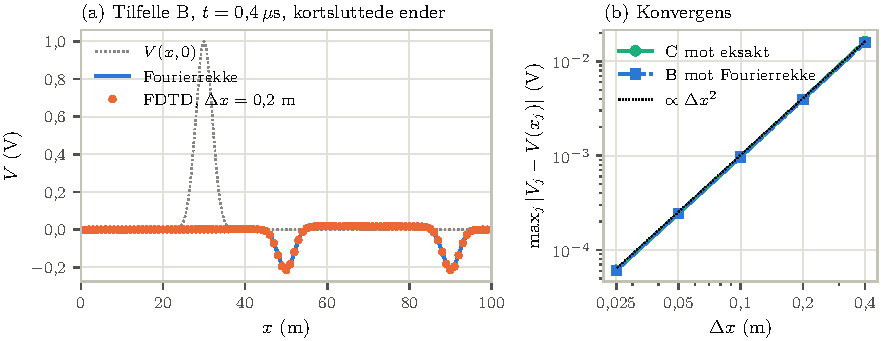
\includegraphics[width=\textwidth]{figurer/verifisering.pdf}
  \caption{(a) FDTD-løsning og Fourier-rekke for tilfelle B med kortsluttede
    ender ved $t = \SI{0.4}{\micro\second}$. (b) Største feil som funksjon av
    $\Delta x$ med $r = 0{,}5$. Den stiplede linja har stigningstall 2.}
  \label{fig:verifisering}
\end{figure}

Tabell~\ref{tab:konvergens} viser største absolutte feil for fem gitteravstander.
Feilen deles på fire hver gang $\Delta x$ halveres. Den observerte ordenen,
$p = \log_2(e_{\Delta x}/e_{\Delta x/2})$, nærmer seg 2,00 i begge testene.

\begin{table}[H]
  \centering
  \caption{Største absolutte feil (\si{\volt}) og observert konvergensorden $p$.}
  \label{tab:konvergens}
  \begin{tabular}{ccccc}
    \toprule
    & \multicolumn{2}{c}{C mot eksakt løsning} & \multicolumn{2}{c}{B mot Fourier-rekke} \\
    \cmidrule(lr){2-3}\cmidrule(lr){4-5}
    $\Delta x$ (\si{\metre}) & Feil & $p$ & Feil & $p$ \\
    \midrule
    \tabellrader{tabeller/konvergens.tex}
    \bottomrule
  \end{tabular}
\end{table}

Energibalansen \eqref{eq:energi} gir en fjerde kontroll. Programmet summerer lagret
energi og integrerer effekttapet. Summen skal være konstant.
Tabell~\ref{tab:pulsmaal} viser at det relative avviket er høyst
$\num{3.3e-5}$ i pulssimuleringene.

\subsection{Dispersjon for modellinjene}\label{sec:disp_res}
Figur~\ref{fig:dispersjon} viser $\alpha$, $v_p$ og $v_g$ for tilfellene A--D,
beregnet fra \eqref{eq:gamma}, \eqref{eq:vp} og \eqref{eq:vg}.

\begin{figure}[!htb]
  \centering
  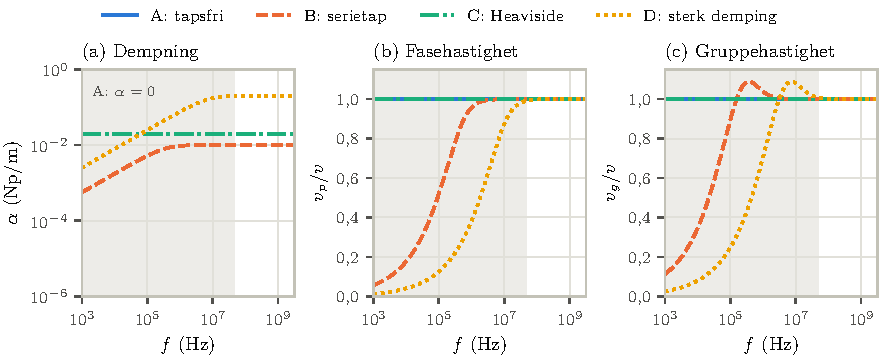
\includegraphics[width=\textwidth]{figurer/dispersjon_modell.pdf}
  \caption{Dempningskonstant, fasehastighet og gruppehastighet for tilfellene
    A--D. Det grå feltet dekker frekvensene som inneholder
    gaussiske pulser med $\sigma_x = \SI{2}{\metre}$ (spektrum over 1\,\% av
    maksimum, $f < \SI{\fpuls}{\mega\hertz}$).}
  \label{fig:dispersjon}
\end{figure}

For tilfelle A og C er $v_p = v_g = v$ ved alle frekvenser. I tilfelle C er
dempningen konstant, $\alpha = \sqrt{RG} = \SI{0.02}{Np\per\metre}$. For
tilfelle B og D stiger $\alpha$ med frekvensen mot grenseverdien $R/(2Z_0)$ fra
\eqref{eq:lavtap}. Fasehastigheten går fra null ved lave frekvenser til $v$ ved
høye frekvenser, med stigningstall $\tfrac12$ i log-log-plott i
lavfrekvensområdet, som i \eqref{eq:diffregime}. Overgangen skjer rundt
$\omega \approx R/L$, som er \SI{0.64}{\mega\hertz} for B og
\SI{13}{\mega\hertz} for D.

Gruppehastigheten er større enn $v$ i et smalt bånd. Med $G = 0$ avhenger
$v_g/v$ bare av $\omega L/R$. Maksimum er $v_g = \num{\vgmaks}\,v$ ved
$\omega = \num{\wvgmaks}\,R/L$.

\subsection{Pulsforplantning}\label{sec:puls}
En gaussisk puls med amplitude \SI{1}{\volt} og standardavvik
$\sigma_x = \SI{2}{\metre}$ starter i $x = \SI{100}{\metre}$ som en høyregående
bølge, $I(x,0) = V(x,0)/Z_0$. Linja er \SI{300}{\metre} lang og avsluttet med
$Z_0$ i begge ender. Simuleringen bruker $\Delta x = \SI{5}{\centi\metre}$ og
$r = 0{,}9$. Figur~\ref{fig:puls} viser pulsen hver
\SI{0.1}{\micro\second}.

\begin{figure}[!htb]
  \centering
  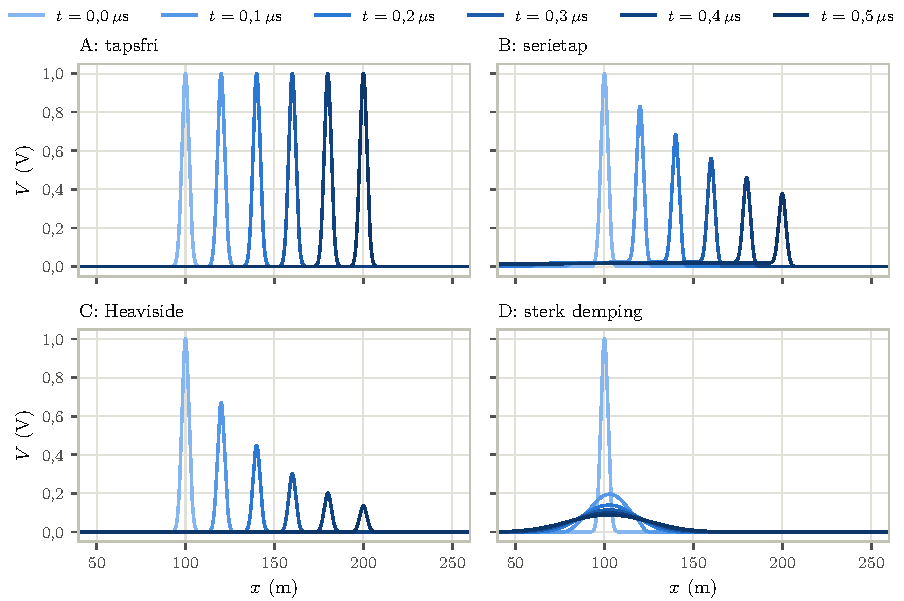
\includegraphics[width=\textwidth]{figurer/puls_bilder.pdf}
  \caption{Spenningen langs linja til seks tidspunkter for tilfellene A--D.}
  \label{fig:puls}
\end{figure}

Figur~\ref{fig:pulsmaal} og tabell~\ref{tab:pulsmaal} viser fire mål på pulsen:
toppverdi, halvverdibredde, ladning $Q = \int CV\,\dd x$ og energi $E$.

\begin{figure}[!htb]
  \centering
  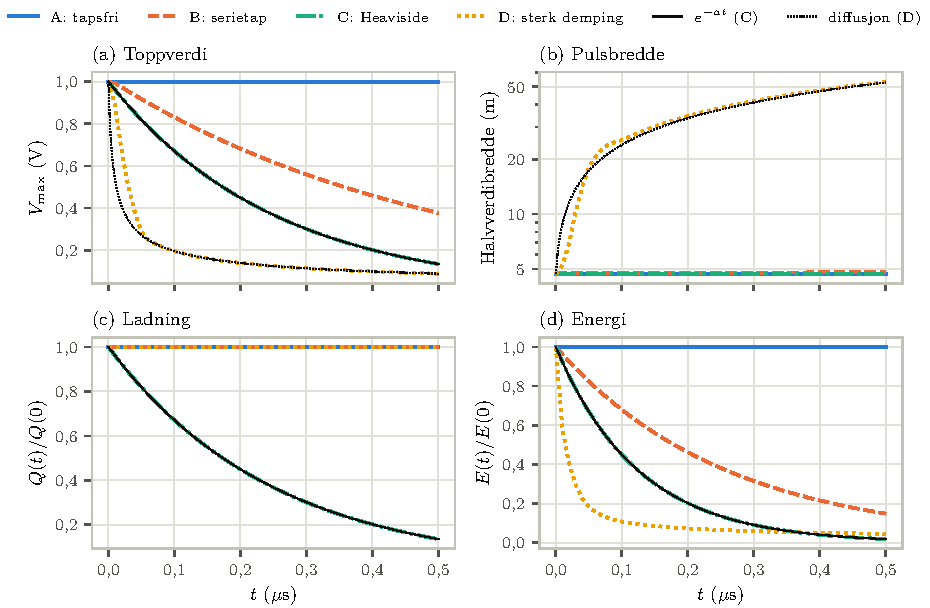
\includegraphics[width=\textwidth]{figurer/puls_maal.pdf}
  \caption{Toppverdi, halvverdibredde, ladning og energi som funksjon av tid. De
    tynne svarte kurvene er teori: $e^{-at}$, $e^{-(G/C)t}$ og $e^{-2at}$ for
    tilfelle C, og diffusjon av en gaussisk puls for tilfelle D.}
  \label{fig:pulsmaal}
\end{figure}

\begin{table}[H]
  \centering
  \caption{Pulsmål ved $t = \SI{0.5}{\micro\second}$. Startverdiene er
    \SI{1}{\volt} og \SI{4.71}{\metre}. Siste kolonne er største relative avvik
    i energibalansen, $\max|E + W_{\text{tap}} - E_0|/E_0$.}
  \label{tab:pulsmaal}
  \begin{tabular}{lccccc}
    \toprule
    Tilfelle & $V_{\max}$ (\si{\volt}) & Bredde (\si{\metre}) & $Q/Q_0$ & $E/E_0$ &
    Avvik energi \\
    \midrule
    \tabellrader{tabeller/pulsmaal.tex}
    \bottomrule
  \end{tabular}
\end{table}

Resultatene for hvert tilfelle:
\begin{itemize}
  \item \textbf{A (tapsfri):} Pulsen beveger seg \SI{100}{\metre} på
        \SI{0.5}{\micro\second} uten å endre form. Farten er
        $v = \SI{2e8}{\metre\per\second}$.
  \item \textbf{B (serietap):} Toppverdien faller til \SI{\toppB}{\volt}, litt
        over $e^{-at} = \num{\toppBteori}$. Bredden øker bare fra \SI{4.71}{\metre} til
        \SI{4.8}{\metre}, men pulsen legger igjen en lang, lav hale. Ladningen er
        bevart ($Q/Q_0 = 0{,}999$), mens energien faller til 15\,\%.
  \item \textbf{C (Heaviside):} Pulsen beholder formen og bredden. Toppverdien
        følger $e^{-at} = e^{-2} = \num{\toppC}$. Største avvik fra den eksakte
        løsningen \eqref{eq:heavisideloesning} er \SI{\feilC}{\volt}.
        Ladningen følger $e^{-(G/C)t}$ og energien $e^{-2at}$.
  \item \textbf{D (sterk demping):} Bølgedelen dempes med $e^{-at}$ og er nesten
        borte etter \SI{0.1}{\micro\second}. Det som er igjen, er en bred, lav klump som
        vokser i bredde som $\sqrt{t}$. Bredden etter \SI{0.5}{\micro\second} er
        \SI{53.4}{\metre}, mot \SI{52.9}{\metre} for ren diffusjon med
        $D = 1/(RC) = \SI{\DD}{\metre\squared\per\second}$. Ladningen er bevart.
\end{itemize}

\subsection{Moder på en endelig linje}\label{sec:moder}
Figur~\ref{fig:moder} viser røttene \eqref{eq:rotter} for de 20 første modene på en
kortsluttet linje med $\ell = \SI{100}{\metre}$.

\begin{figure}[!htb]
  \centering
  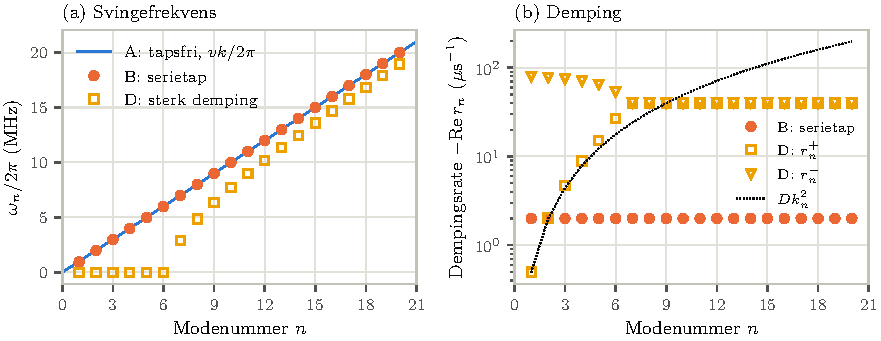
\includegraphics[width=\textwidth]{figurer/moder.pdf}
  \caption{(a) Svingefrekvens og (b) dempingsrate for modene på en kortsluttet
    linje med lengde \SI{100}{\metre}. For tilfelle D viser (b) begge røttene
    $r_n^{\pm}$. Den stiplede kurven er $Dk_n^2$ fra \eqref{eq:langsom}.}
  \label{fig:moder}
\end{figure}

For tilfelle B ligger svingefrekvensene rett under den tapsfrie verdien
$vk_n/(2\pi)$, og alle modene dempes med $a = \SI{\aB}{\per\second}$. For
tilfelle D er $n_c = \num{\ncD}$. Modene $n = 1$ til 6 svinger derfor ikke. De har én
rask og én langsom rot, og den langsomme følger $Dk_n^2$. Fra $n = 7$ svinger
modene, og alle dempes med $a = \SI{\aD}{\per\second}$. Figur~\ref{fig:moder}a
viser altså dispersjonsrelasjonen \eqref{eq:tidsdispersjon} for diskrete
bølgetall.

\subsection{Refleksjoner fra kilde og last}\label{sec:refl_res}
En spenningskilde med stigetid \SI{10}{\nano\second} og $V_0 = \SI{1}{\volt}$
kobles til en linje med lengde \SI{100}{\metre}. Løpetiden er
$T = \SI{0.5}{\micro\second}$. Figur~\ref{fig:refleksjon} viser spenningen over
lasten.

\begin{figure}[!htb]
  \centering
  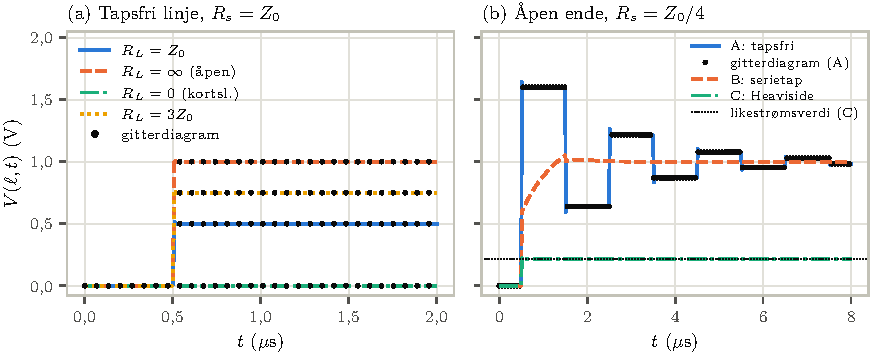
\includegraphics[width=\textwidth]{figurer/refleksjon.pdf}
  \caption{Spenningen over lasten ved et sprang på \SI{1}{\volt}. (a) Tapsfri
    linje med tilpasset kilde og fire laster. (b) Åpen ende og kilde med
    $R_s = Z_0/4 = \SI{12.5}{\ohm}$ for tilfellene A, B og C. Svarte punkter er
    gitterdiagrammet \eqref{eq:gitter}.}
  \label{fig:refleksjon}
\end{figure}

I figur~\ref{fig:refleksjon}a er kilden tilpasset, så bare én refleksjon oppstår.
Lastspenningen blir $\tfrac12(1 + \Gamma_L)$\,\si{\volt}: \SI{0.5}{\volt} for
$R_L = Z_0$, \SI{1}{\volt} for åpen ende, \SI{0}{\volt} for kortslutning og
\SI{0.75}{\volt} for $R_L = 3Z_0$. I figur~\ref{fig:refleksjon}b er
$\Gamma_s = -0{,}6$ og $\Gamma_L = 1$. Den tapsfrie linja ringer rundt
\SI{1}{\volt} med første topp \SI{1.6}{\volt}, og hver rundtur reduserer
avviket med faktoren $0{,}6$. Simuleringen og gitterdiagrammet faller sammen.
Serietapet i tilfelle B demper ringingen, og spenningen kryper mot \SI{1}{\volt}.
Lekkasjen i tilfelle C gir en likestrømsverdi på bare \SI{\VLdc}{\volt}, fordi
strøm lekker ut langs linja.

\subsection{Fra bølge til diffusjon}\label{sec:bolgediff}
Figur~\ref{fig:diffusjon}a viser sprangresponsen \SI{50}{\metre} fra kilden for
fire verdier av $R$, med $G = 0$. De heltrukne kurvene er Laplace-løsningen, de
stiplede er diffusjonsgrensen \eqref{eq:erfc}, og punktene er FDTD-løsningen
for $R = \SI{20}{\ohm\per\metre}$.

\begin{figure}[!htb]
  \centering
  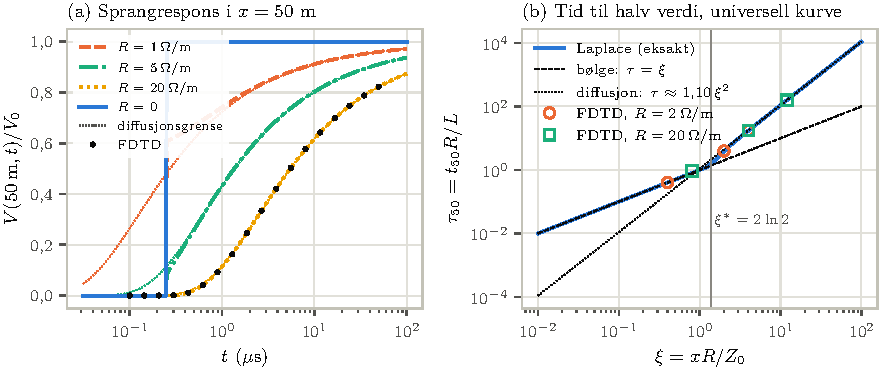
\includegraphics[width=\textwidth]{figurer/diffusjon.pdf}
  \caption{(a) Sprangrespons \SI{50}{\metre} fra en ideell spenningskilde. (b)
    Tid til halv verdi i dimensjonsløse variable \eqref{eq:skalering}. Kurven er
    beregnet med Laplace-løsningen. Punktene er FDTD-simuleringer med to ulike
    serietap.}
  \label{fig:diffusjon}
\end{figure}

For $R = 0$ kommer hele spranget fram etter \SI{0.25}{\micro\second}. For
$R = \SI{1}{\ohm\per\metre}$ er fronthoppet $e^{-0{,}5} = 0{,}61$, og resten kommer
gradvis. For $R = \SI{20}{\ohm\per\metre}$ er fronthoppet bare
$\num{\frontD}$. Spenningen når halv verdi etter \SI{\tfemtiD}{\micro\second},
og diffusjonsformelen \eqref{eq:kvadratlov} gir \SI{\tfemtiDdiff}{\micro\second}.
FDTD-løsningen og Laplace-løsningen stemmer overens.

Figur~\ref{fig:diffusjon}b viser $\tau_{50}$ som funksjon av $\xi$. Kurven følger
bølgegrensen $\tau_{50} = \xi$ eksakt opp til $\xi^* = 2\ln 2 = 1{,}39$, som
forutsagt av \eqref{eq:xstjerne}. Der knekker den og nærmer seg kvadratloven
$\tau_{50} \approx 1{,}10\,\xi^2$. Punktene fra FDTD-simuleringene med
$R = \SI{2}{\ohm\per\metre}$ og $R = \SI{20}{\ohm\per\metre}$ ligger på den samme
kurven.

\subsection{Anvendelse: telefonlinjer og pupinisering}\label{sec:telefon}
Figur~\ref{fig:telefon} og tabell~\ref{tab:telefon} sammenlikner
telefonkabelen fra kapittel~\ref{sec:verktoy} med og uten pupinspoler. Den
tredje linja har induktansen som Heaviside-betingelsen krever,
$L = RC/G = \SI{\LHeaviside}{\henry\per\kilo\metre}$.

\begin{figure}[!htb]
  \centering
  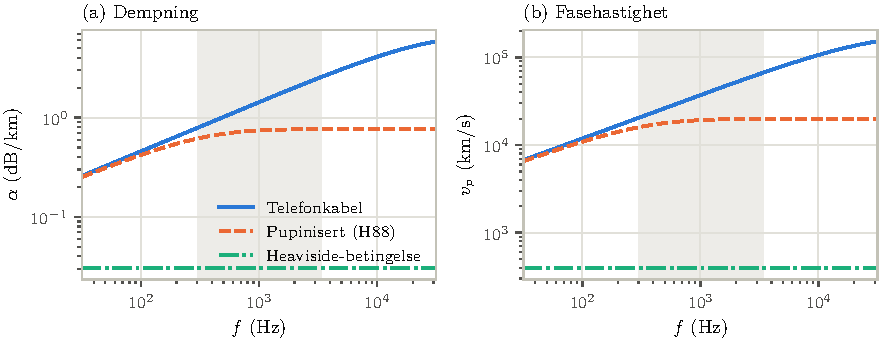
\includegraphics[width=\textwidth]{figurer/telefonlinje.pdf}
  \caption{Dempning og fasehastighet for en telefonkabel (24~AWG) uten og med
    pupinspoler (H88), og med induktansen som oppfyller Heaviside-betingelsen.
    Det grå feltet er talebåndet \SIrange{300}{3400}{\hertz}.}
  \label{fig:telefon}
\end{figure}

\begin{table}[H]
  \centering
  \small
  \caption{Dempning og fasehastighet for telefonkabelen i talebåndet.}
  \label{tab:telefon}
  \begin{tabular}{lccccccc}
    \toprule
    & & \multicolumn{3}{c}{$\alpha$ (\si{\deci\bel\per\kilo\metre})} &
      \multicolumn{3}{c}{$v_p$ (\si{\kilo\metre\per\second})} \\
    \cmidrule(lr){3-5}\cmidrule(lr){6-8}
    Linje & $L$ (\si{\milli\henry\per\kilo\metre}) & \SI{300}{\hertz} & \SI{1}{\kilo\hertz} &
      \SI{3.4}{\kilo\hertz} & \SI{300}{\hertz} & \SI{1}{\kilo\hertz} & \SI{3.4}{\kilo\hertz} \\
    \midrule
    \tabellrader{tabeller/telefon.tex}
    \bottomrule
  \end{tabular}
\end{table}

Uten spoler er $\omega L \ll R$ i hele talebåndet, og kabelen er i
diffusjonsgrensen \eqref{eq:diffregime}. Dempningen stiger fra
\SI{0.79}{\deci\bel\per\kilo\metre} til \SI{2.57}{\deci\bel\per\kilo\metre}, en
forskjell på \SI{\dalfaUten}{\deci\bel\per\kilo\metre}. Over \SI{10}{\kilo\metre}
kommer frekvensene \SI{300}{\hertz} og \SI{3.4}{\kilo\hertz} fram med
\SI{\dtauUten}{\milli\second} forskjell i gruppeforsinkelse. Med spoler er
$\omega L > R$ over omtrent \SI{560}{\hertz}. Dempningen blir nesten flat, med
en variasjon på bare \SI{\dalfaPupin}{\deci\bel\per\kilo\metre}, og
forsinkelsesforskjellen faller til \SI{\dtauPupin}{\milli\second}. Full
Heaviside-betingelse ville krevd omtrent 2500 ganger mer induktans enn
pupiniseringen gir. En slik linje ville hatt svært lav dempning, men også
bølgefarten \SI{397}{\kilo\metre\per\second}, som gir \SI{25}{\milli\second}
forsinkelse over \SI{10}{\kilo\metre}.

% ==========================================================================
\section{Diskusjon}\label{sec:diskusjon}
% ==========================================================================

\subsection{Nøyaktighet og gyldighet}
Løseren er testet mot tre uavhengige analytiske løsninger og mot energibalansen.
Alle testene gir samsvar innenfor forventet nøyaktighet. Konvergensordenen er
2,00, som teorien for sentrale differanser forutsier. At to ulike analytiske
løsninger gir samme orden, tyder på at randbetingelsene og startsteget ikke
reduserer nøyaktigheten. Feilen i pulssimuleringene er av størrelsesorden
$10^{-5}$ av amplituden. Den er derfor langt mindre enn de fysiske effektene
rapporten diskuterer. Den numeriske dispersjonen \eqref{eq:numvp} kunne i
prinsippet blitt forvekslet med fysisk dispersjon. Med $r = 0{,}9$ og fin
oppløsning er den imidlertid under $10^{-5}$, og tilfelle A og C viser ingen
synlig formendring.

Laplace-løsningen med Talbot-inversjon stemmer med erfc-løsningen til åtte
desimaler når $L$ er nær null. Den brukes derfor som fasit for den universelle
kurven i figur~\ref{fig:diffusjon}b.

\subsection{Tap, dispersjon og forvrengning}
Resultatene viser to ulike mekanismer for forvrengning. Når $\alpha$ øker med
frekvensen, fjernes de høye frekvensene først, og pulsen blir bredere og
lavere. Når $v_p$ varierer med frekvensen, kommer komponentene ut av fase.
I tilfelle B ligger pulsspekteret for det meste over overgangsfrekvensen
$R/L$ (figur~\ref{fig:dispersjon}). Dispersjonen er derfor svak, og pulsen
beholder nesten bredden. De laveste frekvensene går likevel saktere og dempes
annerledes. De havner i halen bak pulsen.

Ladningsbalansen \eqref{eq:ladning} gir en enkel forklaring på halen. Serietap
fjerner energi, men ikke ladning. Når pulsen blir lavere, må ladningen den mister
bli liggende igjen på linja. I tilfelle C lekker ladningen ut gjennom $G$ med
nøyaktig samme rate som toppen avtar. Derfor blir det ingen hale. Dette er en
fysisk tolkning av Heaviside-betingelsen: Serietapet og lekkasjen balanserer
hverandre, slik at spenning og strøm i pulsen dempes i samme takt og forholdet
$V/I = Z_0$ bevares.

Toppverdien i tilfelle B avtar litt langsommere enn $e^{-at}$. Forklaringen er
at $e^{-at}$ bare gjelder bølgefronten \eqref{eq:front}. En glatt puls får et
bidrag fra halen som ligger rett bak toppen.

\subsection{Gruppehastighet større enn bølgefarten}
Figur~\ref{fig:dispersjon}c viser at $v_g$ kan bli opptil 8,9\,\% større enn $v$.
Dette ser ut til å stride mot at telegraflikningen er hyperbolsk. Laplace-analysen
viser likevel at ingenting kommer fram før $t = x/v$ \eqref{eq:front}.
Motsetningen løses ved at gruppehastigheten bare beskriver omhyllingskurven til
en smal frekvensgruppe når dempningen er svak over en bølgelengde. I båndet der
$v_g > v$, er $\omega \approx R/L$, og dempningen er sterk. Omhyllingskurven
endrer da form underveis, og toppen kan tilsynelatende flytte seg raskere enn
signalet. Den fysiske grensen er fronthastigheten, og den er $v$.

\subsection{Bølge eller diffusjon}
Skaleringsanalysen \eqref{eq:skalering} gir et enkelt kriterium for hvilken
oppførsel som dominerer. Lengdeskalaen $Z_0/R$ skiller de to områdene. Kortere
avstander gir bølgeoppførsel med forsinkelse $x/v$. Lengre avstander gir diffusjon
med forsinkelse proporsjonal med $x^2$. Tidsskalaen $L/R$ skiller på samme måte
korte og lange tider. Modeanalysen i figur~\ref{fig:moder} viser det samme i
frekvensdomenet: Lange bølger ($vk < |b|$) diffunderer, mens korte bølger svinger.

For den transatlantiske kabelen var $R$ stor og $L$ liten, så $Z_0/R$ var mye
kortere enn kabellengden. Signalet kom derfor fram ved diffusjon, og
forsinkelsen fulgte Thomsons kvadratlov \cite{thomson1855}. Løsningen var ikke
lavere motstand alene, men ekstra induktans. Da øker $Z_0/R$, og en større del
av linja oppfører seg som en bølgeleder. Telefonanalysen viser effekten
kvantitativt. Pupinisering flytter talebåndet fra diffusjonsgrensen til
bølgegrensen. Dempningen blir lavere og nesten uavhengig av frekvensen.

\subsection{Modellens begrensninger}
Modellen antar konstante parametre. I virkelige kabler øker $R$ med
$\sqrt{f}$ på grunn av skinneffekten, og $G$ øker med frekvensen på grunn av
dielektriske tap. Disse effektene gir ekstra dispersjon ved høye frekvenser.
Heaviside-betingelsen kan da bare oppfylles i et begrenset frekvensbånd. Pupinspoler
er diskrete komponenter. En linje med spoler med jevne mellomrom virker som et
lavpassfilter med en øvre grensefrekvens. Denne grensen kommer ikke fram i en
modell med jevnt fordelt induktans. For spoler $L_s$ med avstand $d$ er
grensefrekvensen $f_c = 1/(\pi\sqrt{L_sCd})$ \cite{pozar2012}. For H88-pupinisering
gir det $f_c \approx \SI{3.5}{\kilo\hertz}$, like over talebåndet. Telefonkabelens parametre i tabell~\ref{tab:telefon}
er typiske verdier og vil variere mellom kabeltyper.

% ==========================================================================
\section{Konklusjon}\label{sec:konklusjon}
% ==========================================================================

Telegraflikningen følger direkte av Kirchhoffs lover for en linje med fordelte
parametre. Den er en dempet bølgelikning som inneholder bølgelikningen og
varmelikningen som spesialtilfeller.

Tapene gjør linja dispersiv. Ved høye frekvenser er linja nesten
dispersjonsfri, mens den ved lave frekvenser oppfører seg som et
diffusjonssystem med $v_p \propto \sqrt{\omega}$. Linjer som oppfyller
Heaviside-betingelsen $R/L = G/C$, er et unntak: Alle frekvenser dempes og
forsinkes likt, og pulser overføres uten forvrengning. Simuleringene bekrefter
dette. Serietap alene gir en puls med lang hale, fordi ladningen blir liggende
igjen på linja.

Overgangen fra bølge til diffusjon følger én universell kurve i variablene
$xR/Z_0$ og $tR/L$. Opp til $x^* = 2\ln 2\,Z_0/R$ er forsinkelsen $x/v$, og langt
unna vokser den som $x^2RC$. Gruppehastigheten kan overstige $v$, men
bølgefronten beveger seg aldri raskere enn $v$.

Den numeriske løseren er andre ordens nøyaktig og samsvarer med alle de
analytiske løsningene. Analysen av telefonkabelen viser at ekstra induktans
flytter talebåndet fra diffusjonsområdet til bølgeområdet. Det forklarer hvorfor
pupinisering gjorde taleoverføring over lange avstander mulig.

% ==========================================================================
\begin{thebibliography}{99}
% ==========================================================================
\bibitem{pozar2012}
D. M. Pozar, \emph{Microwave Engineering}, 4. utg. Hoboken, NJ: Wiley, 2012.

\bibitem{thomson1855}
W. Thomson, «On the theory of the electric telegraph», \emph{Proceedings of the
Royal Society of London}, bd. 7, s. 382--399, 1855.

\bibitem{heaviside1893}
O. Heaviside, \emph{Electromagnetic Theory}, bd. 1. London: The Electrician
Printing and Publishing Company, 1893.

\bibitem{nahin2002}
P. J. Nahin, \emph{Oliver Heaviside: The Life, Work, and Times of an Electrical
Genius of the Victorian Age}. Baltimore: Johns Hopkins University Press, 2002.

\bibitem{kreyszig2011}
E. Kreyszig, \emph{Advanced Engineering Mathematics}, 10. utg. Hoboken, NJ:
Wiley, 2011.

\bibitem{strauss2008}
W. A. Strauss, \emph{Partial Differential Equations: An Introduction}, 2. utg.
Hoboken, NJ: Wiley, 2008.

\bibitem{paul2008}
C. R. Paul, \emph{Analysis of Multiconductor Transmission Lines}, 2. utg.
Hoboken, NJ: Wiley--IEEE Press, 2008.

\bibitem{taflove2005}
A. Taflove og S. C. Hagness, \emph{Computational Electrodynamics: The
Finite-Difference Time-Domain Method}, 3. utg. Boston: Artech House, 2005.

\bibitem{abate2004}
J. Abate og P. P. Valkó, «Multi-precision Laplace transform inversion»,
\emph{International Journal for Numerical Methods in Engineering}, bd. 60,
nr. 5, s. 979--993, 2004.

\bibitem{reeve1995}
W. D. Reeve, \emph{Subscriber Loop Signaling and Transmission Handbook}.
New York: IEEE Press, 1995.

\bibitem{numpy}
C. R. Harris mfl., «Array programming with NumPy», \emph{Nature}, bd. 585,
s. 357--362, 2020.

\bibitem{scipy}
P. Virtanen mfl., «SciPy 1.0: Fundamental algorithms for scientific computing
in Python», \emph{Nature Methods}, bd. 17, s. 261--272, 2020.

\bibitem{matplotlib}
J. D. Hunter, «Matplotlib: A 2D graphics environment», \emph{Computing in
Science \& Engineering}, bd. 9, nr. 3, s. 90--95, 2007.
\end{thebibliography}

% ==========================================================================
\clearpage
\section*{Vedlegg A: Programkode}\label{app:kode}
\addcontentsline{toc}{section}{Vedlegg A: Programkode}
\setcounter{table}{0}
\renewcommand{\thetable}{A.\arabic{table}}
% ==========================================================================

Programkoden ligger i mappa \texttt{kode/}. Tabell~\ref{tab:filer} viser filene.
Alle figurer og tabeller i rapporten lages på nytt med kommandoen
\texttt{python lag\_figurer.py}. Kjøretiden er omtrent ett minutt.

\begin{table}[H]
  \centering
  \caption{Filene i programkoden.}
  \label{tab:filer}
  \begin{tabular}{ll}
    \toprule
    Fil & Innhold \\
    \midrule
    \texttt{linje.py}        & Linjeparametre, $\gamma$, $Z_c$, $v_p$, $v_g$ og tilfellene A--D \\
    \texttt{analytisk.py}    & Heaviside-puls, Fourier-rekke, Talbot-inversjon, $t_{50}$, gitterdiagram \\
    \texttt{fdtd.py}         & FDTD-løseren med randbetingelser og energiregnskap \\
    \texttt{stil.py}         & Felles figurstil \\
    \texttt{lag\_figurer.py} & Lager alle figurer og tabeller \\
    \texttt{test\_telegraf.py} & Automatiske tester (pytest) \\
    \bottomrule
  \end{tabular}
\end{table}

\subsection*{A.1 \quad FDTD-løseren (\texttt{fdtd.py})}
\addcontentsline{toc}{subsection}{A.1 \texorpdfstring{\quad}{ } FDTD-løseren}
\lstinputlisting{../kode/fdtd.py}

\subsection*{A.2 \quad Analytiske løsninger (\texttt{analytisk.py})}
\addcontentsline{toc}{subsection}{A.2 \texorpdfstring{\quad}{ } Analytiske løsninger}
\lstinputlisting{../kode/analytisk.py}

\end{document}
